% Options for packages loaded elsewhere
\PassOptionsToPackage{unicode}{hyperref}
\PassOptionsToPackage{hyphens}{url}
\PassOptionsToPackage{dvipsnames,svgnames,x11names}{xcolor}
%
\documentclass[
  letterpaper,
  DIV=11,
  numbers=noendperiod]{scrartcl}

\usepackage{amsmath,amssymb}
\usepackage{iftex}
\ifPDFTeX
  \usepackage[T1]{fontenc}
  \usepackage[utf8]{inputenc}
  \usepackage{textcomp} % provide euro and other symbols
\else % if luatex or xetex
  \usepackage{unicode-math}
  \defaultfontfeatures{Scale=MatchLowercase}
  \defaultfontfeatures[\rmfamily]{Ligatures=TeX,Scale=1}
\fi
\usepackage{lmodern}
\ifPDFTeX\else  
    % xetex/luatex font selection
\fi
% Use upquote if available, for straight quotes in verbatim environments
\IfFileExists{upquote.sty}{\usepackage{upquote}}{}
\IfFileExists{microtype.sty}{% use microtype if available
  \usepackage[]{microtype}
  \UseMicrotypeSet[protrusion]{basicmath} % disable protrusion for tt fonts
}{}
\makeatletter
\@ifundefined{KOMAClassName}{% if non-KOMA class
  \IfFileExists{parskip.sty}{%
    \usepackage{parskip}
  }{% else
    \setlength{\parindent}{0pt}
    \setlength{\parskip}{6pt plus 2pt minus 1pt}}
}{% if KOMA class
  \KOMAoptions{parskip=half}}
\makeatother
\usepackage{xcolor}
\setlength{\emergencystretch}{3em} % prevent overfull lines
\setcounter{secnumdepth}{-\maxdimen} % remove section numbering
% Make \paragraph and \subparagraph free-standing
\ifx\paragraph\undefined\else
  \let\oldparagraph\paragraph
  \renewcommand{\paragraph}[1]{\oldparagraph{#1}\mbox{}}
\fi
\ifx\subparagraph\undefined\else
  \let\oldsubparagraph\subparagraph
  \renewcommand{\subparagraph}[1]{\oldsubparagraph{#1}\mbox{}}
\fi

\usepackage{color}
\usepackage{fancyvrb}
\newcommand{\VerbBar}{|}
\newcommand{\VERB}{\Verb[commandchars=\\\{\}]}
\DefineVerbatimEnvironment{Highlighting}{Verbatim}{commandchars=\\\{\}}
% Add ',fontsize=\small' for more characters per line
\usepackage{framed}
\definecolor{shadecolor}{RGB}{241,243,245}
\newenvironment{Shaded}{\begin{snugshade}}{\end{snugshade}}
\newcommand{\AlertTok}[1]{\textcolor[rgb]{0.68,0.00,0.00}{#1}}
\newcommand{\AnnotationTok}[1]{\textcolor[rgb]{0.37,0.37,0.37}{#1}}
\newcommand{\AttributeTok}[1]{\textcolor[rgb]{0.40,0.45,0.13}{#1}}
\newcommand{\BaseNTok}[1]{\textcolor[rgb]{0.68,0.00,0.00}{#1}}
\newcommand{\BuiltInTok}[1]{\textcolor[rgb]{0.00,0.23,0.31}{#1}}
\newcommand{\CharTok}[1]{\textcolor[rgb]{0.13,0.47,0.30}{#1}}
\newcommand{\CommentTok}[1]{\textcolor[rgb]{0.37,0.37,0.37}{#1}}
\newcommand{\CommentVarTok}[1]{\textcolor[rgb]{0.37,0.37,0.37}{\textit{#1}}}
\newcommand{\ConstantTok}[1]{\textcolor[rgb]{0.56,0.35,0.01}{#1}}
\newcommand{\ControlFlowTok}[1]{\textcolor[rgb]{0.00,0.23,0.31}{#1}}
\newcommand{\DataTypeTok}[1]{\textcolor[rgb]{0.68,0.00,0.00}{#1}}
\newcommand{\DecValTok}[1]{\textcolor[rgb]{0.68,0.00,0.00}{#1}}
\newcommand{\DocumentationTok}[1]{\textcolor[rgb]{0.37,0.37,0.37}{\textit{#1}}}
\newcommand{\ErrorTok}[1]{\textcolor[rgb]{0.68,0.00,0.00}{#1}}
\newcommand{\ExtensionTok}[1]{\textcolor[rgb]{0.00,0.23,0.31}{#1}}
\newcommand{\FloatTok}[1]{\textcolor[rgb]{0.68,0.00,0.00}{#1}}
\newcommand{\FunctionTok}[1]{\textcolor[rgb]{0.28,0.35,0.67}{#1}}
\newcommand{\ImportTok}[1]{\textcolor[rgb]{0.00,0.46,0.62}{#1}}
\newcommand{\InformationTok}[1]{\textcolor[rgb]{0.37,0.37,0.37}{#1}}
\newcommand{\KeywordTok}[1]{\textcolor[rgb]{0.00,0.23,0.31}{#1}}
\newcommand{\NormalTok}[1]{\textcolor[rgb]{0.00,0.23,0.31}{#1}}
\newcommand{\OperatorTok}[1]{\textcolor[rgb]{0.37,0.37,0.37}{#1}}
\newcommand{\OtherTok}[1]{\textcolor[rgb]{0.00,0.23,0.31}{#1}}
\newcommand{\PreprocessorTok}[1]{\textcolor[rgb]{0.68,0.00,0.00}{#1}}
\newcommand{\RegionMarkerTok}[1]{\textcolor[rgb]{0.00,0.23,0.31}{#1}}
\newcommand{\SpecialCharTok}[1]{\textcolor[rgb]{0.37,0.37,0.37}{#1}}
\newcommand{\SpecialStringTok}[1]{\textcolor[rgb]{0.13,0.47,0.30}{#1}}
\newcommand{\StringTok}[1]{\textcolor[rgb]{0.13,0.47,0.30}{#1}}
\newcommand{\VariableTok}[1]{\textcolor[rgb]{0.07,0.07,0.07}{#1}}
\newcommand{\VerbatimStringTok}[1]{\textcolor[rgb]{0.13,0.47,0.30}{#1}}
\newcommand{\WarningTok}[1]{\textcolor[rgb]{0.37,0.37,0.37}{\textit{#1}}}

\providecommand{\tightlist}{%
  \setlength{\itemsep}{0pt}\setlength{\parskip}{0pt}}\usepackage{longtable,booktabs,array}
\usepackage{calc} % for calculating minipage widths
% Correct order of tables after \paragraph or \subparagraph
\usepackage{etoolbox}
\makeatletter
\patchcmd\longtable{\par}{\if@noskipsec\mbox{}\fi\par}{}{}
\makeatother
% Allow footnotes in longtable head/foot
\IfFileExists{footnotehyper.sty}{\usepackage{footnotehyper}}{\usepackage{footnote}}
\makesavenoteenv{longtable}
\usepackage{graphicx}
\makeatletter
\def\maxwidth{\ifdim\Gin@nat@width>\linewidth\linewidth\else\Gin@nat@width\fi}
\def\maxheight{\ifdim\Gin@nat@height>\textheight\textheight\else\Gin@nat@height\fi}
\makeatother
% Scale images if necessary, so that they will not overflow the page
% margins by default, and it is still possible to overwrite the defaults
% using explicit options in \includegraphics[width, height, ...]{}
\setkeys{Gin}{width=\maxwidth,height=\maxheight,keepaspectratio}
% Set default figure placement to htbp
\makeatletter
\def\fps@figure{htbp}
\makeatother

\KOMAoption{captions}{tableheading}
\makeatletter
\makeatother
\makeatletter
\makeatother
\makeatletter
\@ifpackageloaded{caption}{}{\usepackage{caption}}
\AtBeginDocument{%
\ifdefined\contentsname
  \renewcommand*\contentsname{Table of contents}
\else
  \newcommand\contentsname{Table of contents}
\fi
\ifdefined\listfigurename
  \renewcommand*\listfigurename{List of Figures}
\else
  \newcommand\listfigurename{List of Figures}
\fi
\ifdefined\listtablename
  \renewcommand*\listtablename{List of Tables}
\else
  \newcommand\listtablename{List of Tables}
\fi
\ifdefined\figurename
  \renewcommand*\figurename{Figure}
\else
  \newcommand\figurename{Figure}
\fi
\ifdefined\tablename
  \renewcommand*\tablename{Table}
\else
  \newcommand\tablename{Table}
\fi
}
\@ifpackageloaded{float}{}{\usepackage{float}}
\floatstyle{ruled}
\@ifundefined{c@chapter}{\newfloat{codelisting}{h}{lop}}{\newfloat{codelisting}{h}{lop}[chapter]}
\floatname{codelisting}{Listing}
\newcommand*\listoflistings{\listof{codelisting}{List of Listings}}
\makeatother
\makeatletter
\@ifpackageloaded{caption}{}{\usepackage{caption}}
\@ifpackageloaded{subcaption}{}{\usepackage{subcaption}}
\makeatother
\makeatletter
\@ifpackageloaded{tcolorbox}{}{\usepackage[skins,breakable]{tcolorbox}}
\makeatother
\makeatletter
\@ifundefined{shadecolor}{\definecolor{shadecolor}{rgb}{.97, .97, .97}}
\makeatother
\makeatletter
\makeatother
\makeatletter
\makeatother
\ifLuaTeX
  \usepackage{selnolig}  % disable illegal ligatures
\fi
\IfFileExists{bookmark.sty}{\usepackage{bookmark}}{\usepackage{hyperref}}
\IfFileExists{xurl.sty}{\usepackage{xurl}}{} % add URL line breaks if available
\urlstyle{same} % disable monospaced font for URLs
\hypersetup{
  pdftitle={HW 6: R Functions},
  pdfauthor={Alexis Galano (PID: A17628362)},
  colorlinks=true,
  linkcolor={blue},
  filecolor={Maroon},
  citecolor={Blue},
  urlcolor={Blue},
  pdfcreator={LaTeX via pandoc}}

\title{HW 6: R Functions}
\author{Alexis Galano (PID: A17628362)}
\date{2024-01-25}

\begin{document}
\maketitle
\ifdefined\Shaded\renewenvironment{Shaded}{\begin{tcolorbox}[enhanced, frame hidden, interior hidden, borderline west={3pt}{0pt}{shadecolor}, sharp corners, boxrule=0pt, breakable]}{\end{tcolorbox}}\fi

\textbf{R Functions}

\begin{Shaded}
\begin{Highlighting}[]
\CommentTok{\# Can you improve this analysis code?}
\FunctionTok{library}\NormalTok{(bio3d)}
\NormalTok{s1 }\OtherTok{\textless{}{-}} \FunctionTok{read.pdb}\NormalTok{(}\StringTok{"4AKE"}\NormalTok{) }\CommentTok{\# kinase with drug}
\end{Highlighting}
\end{Shaded}

\begin{verbatim}
  Note: Accessing on-line PDB file
\end{verbatim}

\begin{Shaded}
\begin{Highlighting}[]
\NormalTok{s2 }\OtherTok{\textless{}{-}} \FunctionTok{read.pdb}\NormalTok{(}\StringTok{"1AKE"}\NormalTok{) }\CommentTok{\# kinase no drug}
\end{Highlighting}
\end{Shaded}

\begin{verbatim}
  Note: Accessing on-line PDB file
   PDB has ALT records, taking A only, rm.alt=TRUE
\end{verbatim}

\begin{Shaded}
\begin{Highlighting}[]
\NormalTok{s3 }\OtherTok{\textless{}{-}} \FunctionTok{read.pdb}\NormalTok{(}\StringTok{"1E4Y"}\NormalTok{) }\CommentTok{\# kinase with drug}
\end{Highlighting}
\end{Shaded}

\begin{verbatim}
  Note: Accessing on-line PDB file
\end{verbatim}

\begin{Shaded}
\begin{Highlighting}[]
\NormalTok{s1.chainA }\OtherTok{\textless{}{-}} \FunctionTok{trim.pdb}\NormalTok{(s1, }\AttributeTok{chain=}\StringTok{"A"}\NormalTok{, }\AttributeTok{elety=}\StringTok{"CA"}\NormalTok{)}
\NormalTok{s2.chainA }\OtherTok{\textless{}{-}} \FunctionTok{trim.pdb}\NormalTok{(s2, }\AttributeTok{chain=}\StringTok{"A"}\NormalTok{, }\AttributeTok{elety=}\StringTok{"CA"}\NormalTok{)}
\NormalTok{s3.chainA }\OtherTok{\textless{}{-}} \FunctionTok{trim.pdb}\NormalTok{(s1, }\AttributeTok{chain=}\StringTok{"A"}\NormalTok{, }\AttributeTok{elety=}\StringTok{"CA"}\NormalTok{)}

\NormalTok{s1.b }\OtherTok{\textless{}{-}}\NormalTok{ s1.chainA}\SpecialCharTok{$}\NormalTok{atom}\SpecialCharTok{$}\NormalTok{b}
\NormalTok{s2.b }\OtherTok{\textless{}{-}}\NormalTok{ s2.chainA}\SpecialCharTok{$}\NormalTok{atom}\SpecialCharTok{$}\NormalTok{b}
\NormalTok{s3.b }\OtherTok{\textless{}{-}}\NormalTok{ s3.chainA}\SpecialCharTok{$}\NormalTok{atom}\SpecialCharTok{$}\NormalTok{b}

\FunctionTok{plotb3}\NormalTok{(s1.b, }\AttributeTok{sse=}\NormalTok{s1.chainA, }\AttributeTok{typ=}\StringTok{"l"}\NormalTok{, }\AttributeTok{ylab=}\StringTok{"Bfactor"}\NormalTok{)}
\end{Highlighting}
\end{Shaded}

\begin{figure}[H]

{\centering 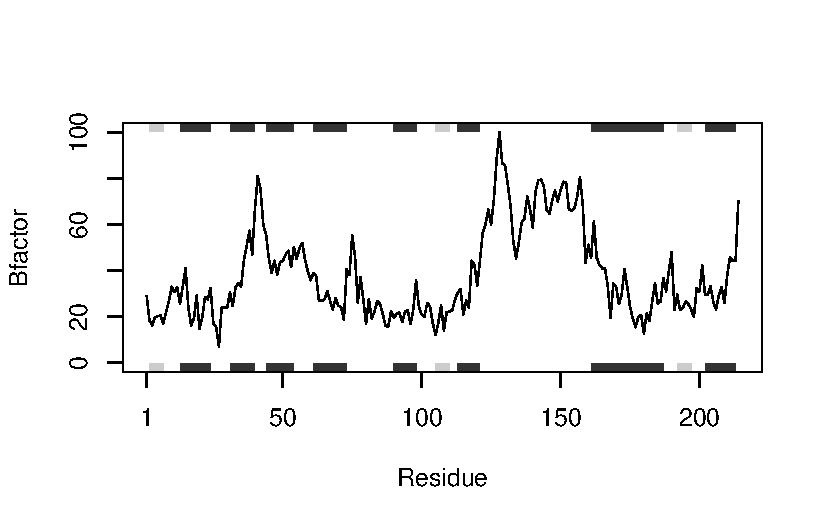
\includegraphics{hw6_turnin_files/figure-pdf/unnamed-chunk-1-1.pdf}

}

\end{figure}

\begin{Shaded}
\begin{Highlighting}[]
\FunctionTok{plotb3}\NormalTok{(s2.b, }\AttributeTok{sse=}\NormalTok{s2.chainA, }\AttributeTok{typ=}\StringTok{"l"}\NormalTok{, }\AttributeTok{ylab=}\StringTok{"Bfactor"}\NormalTok{)}
\end{Highlighting}
\end{Shaded}

\begin{figure}[H]

{\centering 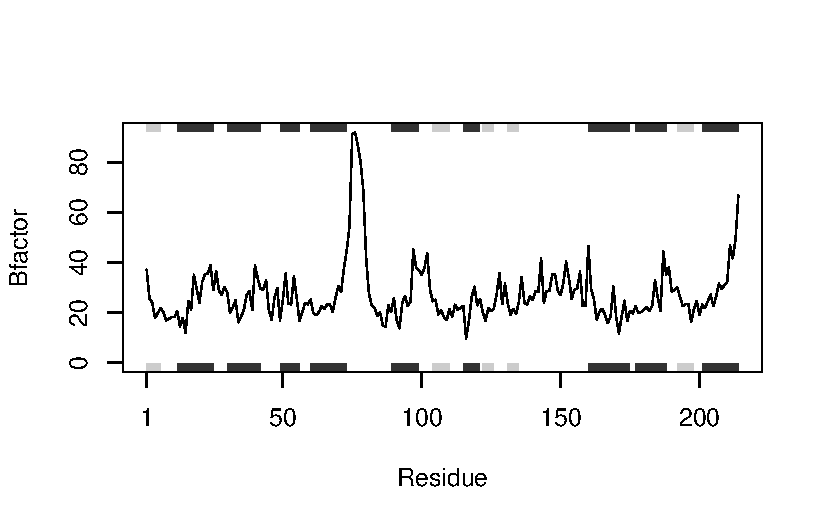
\includegraphics{hw6_turnin_files/figure-pdf/unnamed-chunk-1-2.pdf}

}

\end{figure}

\begin{Shaded}
\begin{Highlighting}[]
\FunctionTok{plotb3}\NormalTok{(s3.b, }\AttributeTok{sse=}\NormalTok{s3.chainA, }\AttributeTok{typ=}\StringTok{"l"}\NormalTok{, }\AttributeTok{ylab=}\StringTok{"Bfactor"}\NormalTok{) }
\end{Highlighting}
\end{Shaded}

\begin{figure}[H]

{\centering 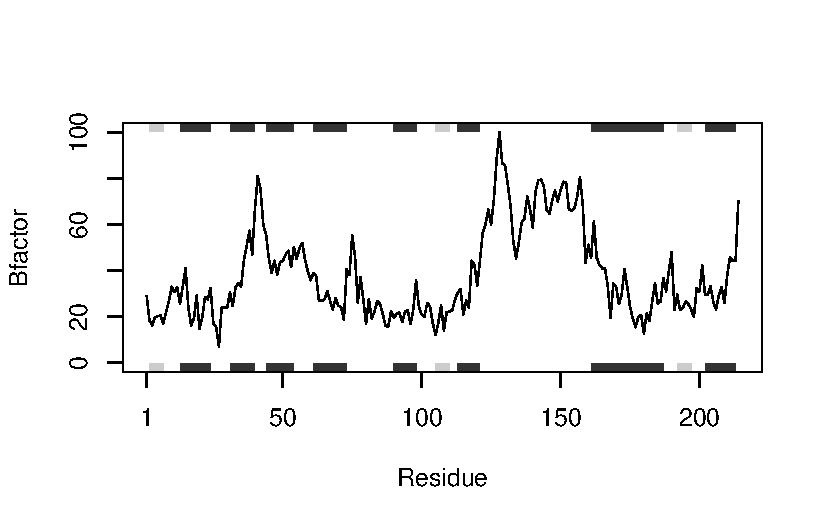
\includegraphics{hw6_turnin_files/figure-pdf/unnamed-chunk-1-3.pdf}

}

\end{figure}

\textbf{Q1. What type of object is returned from the read.pdb()
function?}

\begin{itemize}
\tightlist
\item
  read.pdb() opens a file with a data bank of proteins
\end{itemize}

\textbf{Q2. What does the trim.pdb() function do?}

\begin{itemize}
\tightlist
\item
  trim.pdb() makes a new smaller PDB object with a subset of atoms from
  a given larger PDB object
\end{itemize}

\textbf{Q3. What input parameter would turn off the marginal black and
grey rectangles in the plots and what do they represent in this case?}

\begin{Shaded}
\begin{Highlighting}[]
\FunctionTok{plotb3}\NormalTok{(s1.b, }\AttributeTok{sse=}\NormalTok{s1.chainA, }\AttributeTok{typ=}\StringTok{"l"}\NormalTok{, }\AttributeTok{ylab=}\StringTok{"Bfactor"}\NormalTok{)}
\end{Highlighting}
\end{Shaded}

\begin{figure}[H]

{\centering 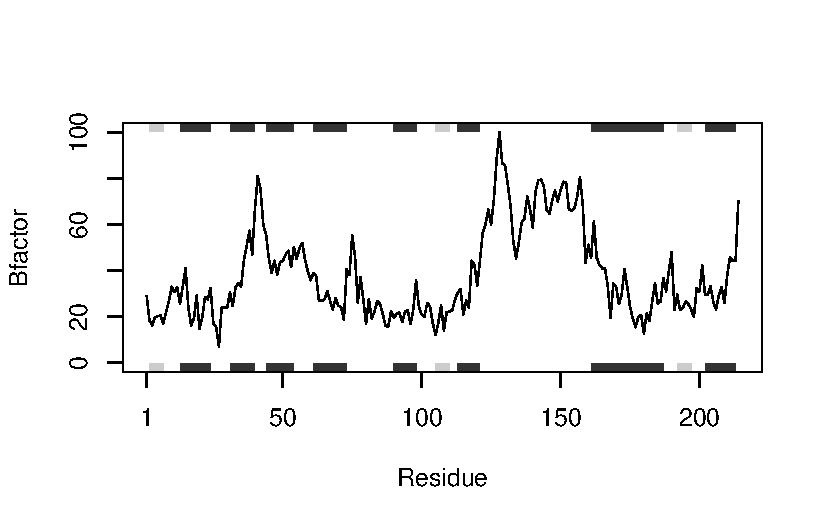
\includegraphics{hw6_turnin_files/figure-pdf/unnamed-chunk-2-1.pdf}

}

\end{figure}

\begin{itemize}
\tightlist
\item
  We can turn off the marginal black and grey rectangles in the plots by
  setting sse=NULL instead of sse=s1.chainA
\end{itemize}

\hypertarget{lets-try-that-below-to-make-sure}{%
\section{Let's try that below to make
sure}\label{lets-try-that-below-to-make-sure}}

\begin{Shaded}
\begin{Highlighting}[]
\FunctionTok{plotb3}\NormalTok{(s1.b, }\AttributeTok{sse=}\ConstantTok{NULL}\NormalTok{, }\AttributeTok{typ=}\StringTok{"l"}\NormalTok{, }\AttributeTok{ylab=}\StringTok{"Bfactor"}\NormalTok{)}
\end{Highlighting}
\end{Shaded}

\begin{figure}[H]

{\centering 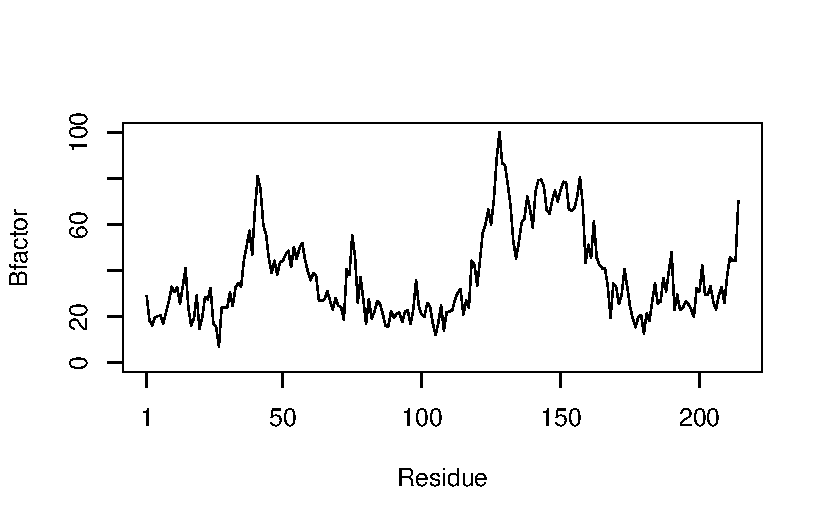
\includegraphics{hw6_turnin_files/figure-pdf/unnamed-chunk-3-1.pdf}

}

\end{figure}

\begin{itemize}
\tightlist
\item
  Yes, we were able to remove the black and white margins by calling
  sse=NULL. These marginal rectangles may show the location of secondary
  structure elements.
\end{itemize}

\textbf{Q4. What would be a better plot to compare across the different
proteins?} - We could use RMSD to compare two or more different proteins
and their structures.

\textbf{Q5. Which proteins are more similar to each other in their
B-factor trends. How could you quantify this?}

\begin{Shaded}
\begin{Highlighting}[]
\NormalTok{hc }\OtherTok{\textless{}{-}} \FunctionTok{hclust}\NormalTok{( }\FunctionTok{dist}\NormalTok{( }\FunctionTok{rbind}\NormalTok{(s1.b, s2.b, s3.b) ) )}
\FunctionTok{plot}\NormalTok{(hc)}
\end{Highlighting}
\end{Shaded}

\begin{figure}[H]

{\centering 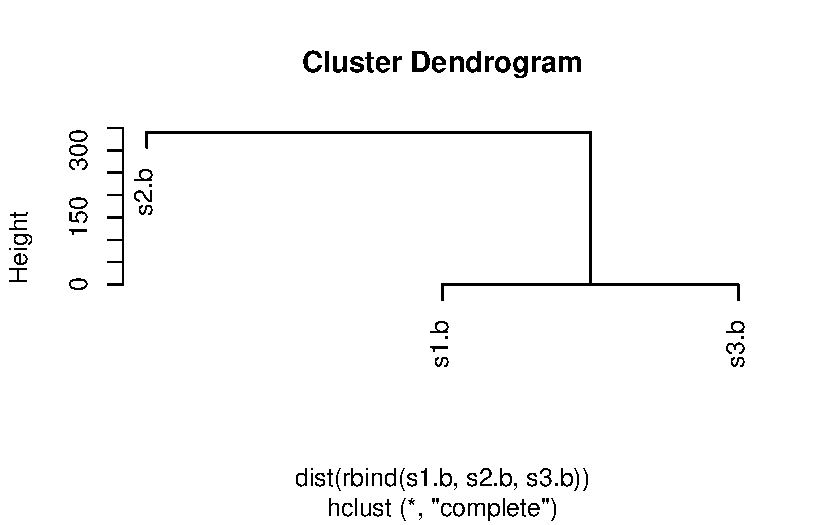
\includegraphics{hw6_turnin_files/figure-pdf/unnamed-chunk-4-1.pdf}

}

\end{figure}

\begin{itemize}
\tightlist
\item
  Based on the dendrogram plot, proteins s1.b and s3.b are more similar
  to each other than to s2.b. This similarity may be due to s1 and s3
  being kinases with drugs whereas s2 kinase goes without a drug.
\end{itemize}

\begin{Shaded}
\begin{Highlighting}[]
\NormalTok{s1 }\OtherTok{\textless{}{-}} \FunctionTok{read.pdb}\NormalTok{(}\StringTok{"4AKE"}\NormalTok{) }\CommentTok{\# kinase with drug}
\end{Highlighting}
\end{Shaded}

\begin{verbatim}
  Note: Accessing on-line PDB file
\end{verbatim}

\begin{verbatim}
Warning in get.pdb(file, path = tempdir(), verbose = FALSE):
C:\Users\argal\AppData\Local\Temp\RtmpSYC6Ek/4AKE.pdb exists. Skipping download
\end{verbatim}

\begin{Shaded}
\begin{Highlighting}[]
\NormalTok{s2 }\OtherTok{\textless{}{-}} \FunctionTok{read.pdb}\NormalTok{(}\StringTok{"1AKE"}\NormalTok{) }\CommentTok{\# kinase no drug}
\end{Highlighting}
\end{Shaded}

\begin{verbatim}
  Note: Accessing on-line PDB file
\end{verbatim}

\begin{verbatim}
Warning in get.pdb(file, path = tempdir(), verbose = FALSE):
C:\Users\argal\AppData\Local\Temp\RtmpSYC6Ek/1AKE.pdb exists. Skipping download
\end{verbatim}

\begin{verbatim}
   PDB has ALT records, taking A only, rm.alt=TRUE
\end{verbatim}

\begin{Shaded}
\begin{Highlighting}[]
\NormalTok{s3 }\OtherTok{\textless{}{-}} \FunctionTok{read.pdb}\NormalTok{(}\StringTok{"1E4Y"}\NormalTok{) }\CommentTok{\# kinase with drug}
\end{Highlighting}
\end{Shaded}

\begin{verbatim}
  Note: Accessing on-line PDB file
\end{verbatim}

\begin{verbatim}
Warning in get.pdb(file, path = tempdir(), verbose = FALSE):
C:\Users\argal\AppData\Local\Temp\RtmpSYC6Ek/1E4Y.pdb exists. Skipping download
\end{verbatim}

\begin{Shaded}
\begin{Highlighting}[]
\NormalTok{s1.chainA }\OtherTok{\textless{}{-}} \FunctionTok{trim.pdb}\NormalTok{(s1, }\AttributeTok{chain=}\StringTok{"A"}\NormalTok{, }\AttributeTok{elety=}\StringTok{"CA"}\NormalTok{)}
\NormalTok{s2.chainA }\OtherTok{\textless{}{-}} \FunctionTok{trim.pdb}\NormalTok{(s2, }\AttributeTok{chain=}\StringTok{"A"}\NormalTok{, }\AttributeTok{elety=}\StringTok{"CA"}\NormalTok{)}
\NormalTok{s3.chainA }\OtherTok{\textless{}{-}} \FunctionTok{trim.pdb}\NormalTok{(s1, }\AttributeTok{chain=}\StringTok{"A"}\NormalTok{, }\AttributeTok{elety=}\StringTok{"CA"}\NormalTok{)}
\NormalTok{s1.b }\OtherTok{\textless{}{-}}\NormalTok{ s1.chainA}\SpecialCharTok{$}\NormalTok{atom}\SpecialCharTok{$}\NormalTok{b}
\NormalTok{s2.b }\OtherTok{\textless{}{-}}\NormalTok{ s2.chainA}\SpecialCharTok{$}\NormalTok{atom}\SpecialCharTok{$}\NormalTok{b}
\NormalTok{s3.b }\OtherTok{\textless{}{-}}\NormalTok{ s3.chainA}\SpecialCharTok{$}\NormalTok{atom}\SpecialCharTok{$}\NormalTok{b}
\FunctionTok{plotb3}\NormalTok{(s1.b, }\AttributeTok{sse=}\NormalTok{s1.chainA, }\AttributeTok{typ=}\StringTok{"l"}\NormalTok{, }\AttributeTok{ylab=}\StringTok{"Bfactor"}\NormalTok{)}
\end{Highlighting}
\end{Shaded}

\begin{figure}[H]

{\centering 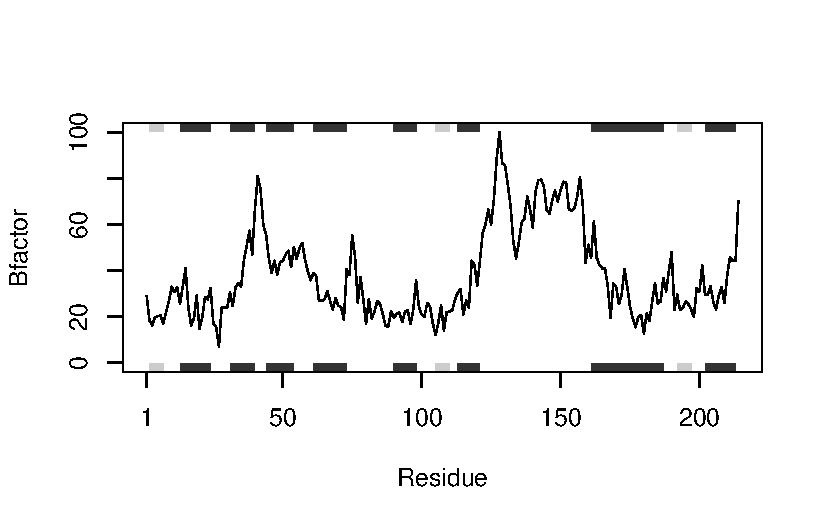
\includegraphics{hw6_turnin_files/figure-pdf/unnamed-chunk-5-1.pdf}

}

\end{figure}

\begin{Shaded}
\begin{Highlighting}[]
\FunctionTok{plotb3}\NormalTok{(s2.b, }\AttributeTok{sse=}\NormalTok{s2.chainA, }\AttributeTok{typ=}\StringTok{"l"}\NormalTok{, }\AttributeTok{ylab=}\StringTok{"Bfactor"}\NormalTok{)}
\end{Highlighting}
\end{Shaded}

\begin{figure}[H]

{\centering 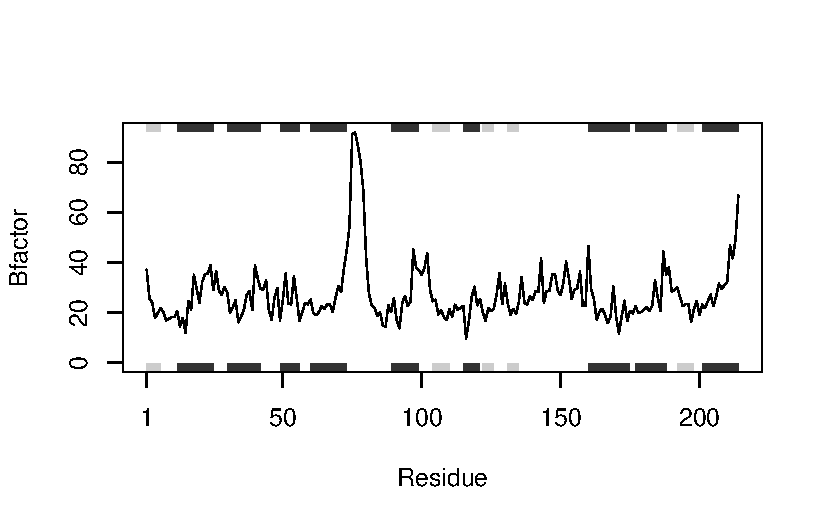
\includegraphics{hw6_turnin_files/figure-pdf/unnamed-chunk-5-2.pdf}

}

\end{figure}

\begin{Shaded}
\begin{Highlighting}[]
\FunctionTok{plotb3}\NormalTok{(s3.b, }\AttributeTok{sse=}\NormalTok{s3.chainA, }\AttributeTok{typ=}\StringTok{"l"}\NormalTok{, }\AttributeTok{ylab=}\StringTok{"Bfactor"}\NormalTok{)}
\end{Highlighting}
\end{Shaded}

\begin{figure}[H]

{\centering 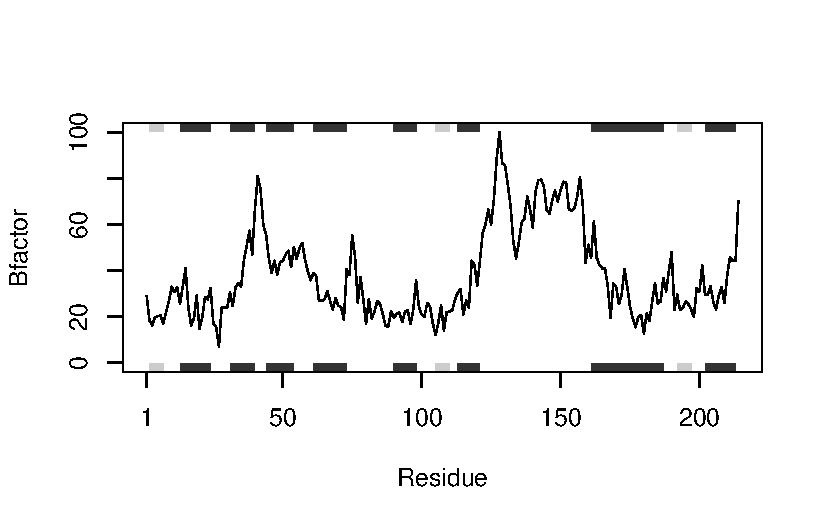
\includegraphics{hw6_turnin_files/figure-pdf/unnamed-chunk-5-3.pdf}

}

\end{figure}

*Q6.\textbf{How would you generalize the original code above to work
with any set of input protein structures?}

\begin{Shaded}
\begin{Highlighting}[]
\CommentTok{\# Original code}

\FunctionTok{library}\NormalTok{(bio3d)}


\NormalTok{s1 }\OtherTok{\textless{}{-}} \FunctionTok{read.pdb}\NormalTok{(}\StringTok{"4AKE"}\NormalTok{) }\CommentTok{\# kinase with drug}
\end{Highlighting}
\end{Shaded}

\begin{verbatim}
  Note: Accessing on-line PDB file
\end{verbatim}

\begin{verbatim}
Warning in get.pdb(file, path = tempdir(), verbose = FALSE):
C:\Users\argal\AppData\Local\Temp\RtmpSYC6Ek/4AKE.pdb exists. Skipping download
\end{verbatim}

\begin{Shaded}
\begin{Highlighting}[]
\NormalTok{s2 }\OtherTok{\textless{}{-}} \FunctionTok{read.pdb}\NormalTok{(}\StringTok{"1AKE"}\NormalTok{) }\CommentTok{\# kinase no drug}
\end{Highlighting}
\end{Shaded}

\begin{verbatim}
  Note: Accessing on-line PDB file
\end{verbatim}

\begin{verbatim}
Warning in get.pdb(file, path = tempdir(), verbose = FALSE):
C:\Users\argal\AppData\Local\Temp\RtmpSYC6Ek/1AKE.pdb exists. Skipping download
\end{verbatim}

\begin{verbatim}
   PDB has ALT records, taking A only, rm.alt=TRUE
\end{verbatim}

\begin{Shaded}
\begin{Highlighting}[]
\NormalTok{s3 }\OtherTok{\textless{}{-}} \FunctionTok{read.pdb}\NormalTok{(}\StringTok{"1E4Y"}\NormalTok{) }\CommentTok{\# kinase with drug}
\end{Highlighting}
\end{Shaded}

\begin{verbatim}
  Note: Accessing on-line PDB file
\end{verbatim}

\begin{verbatim}
Warning in get.pdb(file, path = tempdir(), verbose = FALSE):
C:\Users\argal\AppData\Local\Temp\RtmpSYC6Ek/1E4Y.pdb exists. Skipping download
\end{verbatim}

\begin{Shaded}
\begin{Highlighting}[]
\NormalTok{s1.chainA }\OtherTok{\textless{}{-}} \FunctionTok{trim.pdb}\NormalTok{(s1, }\AttributeTok{chain=}\StringTok{"A"}\NormalTok{, }\AttributeTok{elety=}\StringTok{"CA"}\NormalTok{)}
\NormalTok{s2.chainA }\OtherTok{\textless{}{-}} \FunctionTok{trim.pdb}\NormalTok{(s2, }\AttributeTok{chain=}\StringTok{"A"}\NormalTok{, }\AttributeTok{elety=}\StringTok{"CA"}\NormalTok{)}
\NormalTok{s3.chainA }\OtherTok{\textless{}{-}} \FunctionTok{trim.pdb}\NormalTok{(s1, }\AttributeTok{chain=}\StringTok{"A"}\NormalTok{, }\AttributeTok{elety=}\StringTok{"CA"}\NormalTok{)}

\NormalTok{s1.b }\OtherTok{\textless{}{-}}\NormalTok{ s1.chainA}\SpecialCharTok{$}\NormalTok{atom}\SpecialCharTok{$}\NormalTok{b}
\NormalTok{s2.b }\OtherTok{\textless{}{-}}\NormalTok{ s2.chainA}\SpecialCharTok{$}\NormalTok{atom}\SpecialCharTok{$}\NormalTok{b}
\NormalTok{s3.b }\OtherTok{\textless{}{-}}\NormalTok{ s3.chainA}\SpecialCharTok{$}\NormalTok{atom}\SpecialCharTok{$}\NormalTok{b}

\FunctionTok{plotb3}\NormalTok{(s1.b, }\AttributeTok{sse=}\NormalTok{s1.chainA, }\AttributeTok{typ=}\StringTok{"l"}\NormalTok{, }\AttributeTok{ylab=}\StringTok{"Bfactor"}\NormalTok{)}
\end{Highlighting}
\end{Shaded}

\begin{figure}[H]

{\centering 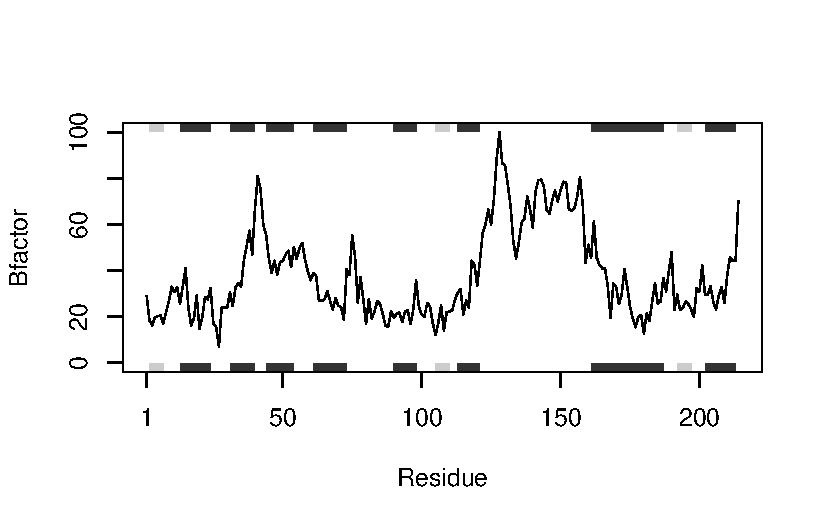
\includegraphics{hw6_turnin_files/figure-pdf/unnamed-chunk-6-1.pdf}

}

\end{figure}

\begin{Shaded}
\begin{Highlighting}[]
\FunctionTok{plotb3}\NormalTok{(s2.b, }\AttributeTok{sse=}\NormalTok{s2.chainA, }\AttributeTok{typ=}\StringTok{"l"}\NormalTok{, }\AttributeTok{ylab=}\StringTok{"Bfactor"}\NormalTok{)}
\end{Highlighting}
\end{Shaded}

\begin{figure}[H]

{\centering 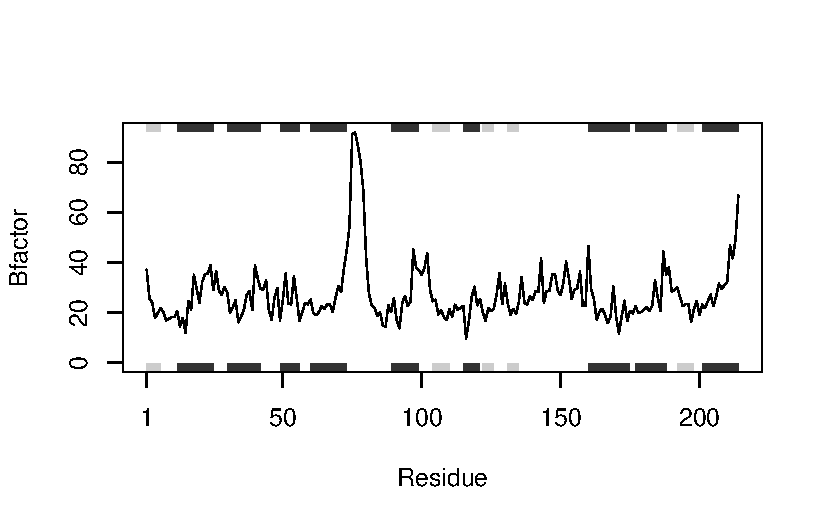
\includegraphics{hw6_turnin_files/figure-pdf/unnamed-chunk-6-2.pdf}

}

\end{figure}

\begin{Shaded}
\begin{Highlighting}[]
\FunctionTok{plotb3}\NormalTok{(s3.b, }\AttributeTok{sse=}\NormalTok{s3.chainA, }\AttributeTok{typ=}\StringTok{"l"}\NormalTok{, }\AttributeTok{ylab=}\StringTok{"Bfactor"}\NormalTok{) }
\end{Highlighting}
\end{Shaded}

\begin{figure}[H]

{\centering 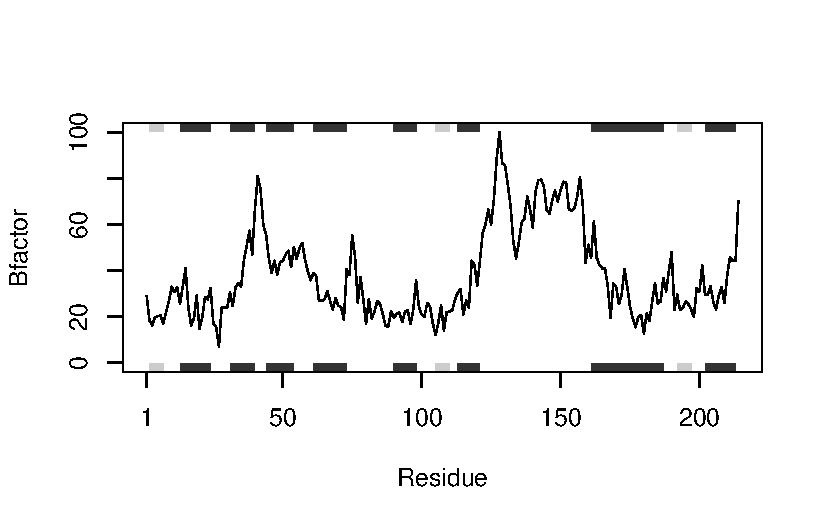
\includegraphics{hw6_turnin_files/figure-pdf/unnamed-chunk-6-3.pdf}

}

\end{figure}

\begin{Shaded}
\begin{Highlighting}[]
\CommentTok{\#We are going to call our function "protein\_analyzer" for its ability to assemble an analysis of a set of three desired protein inputs: prot1, prot2, prot3.}

\NormalTok{protein\_analyzer }\OtherTok{\textless{}{-}} \ControlFlowTok{function}\NormalTok{(prot1, prot2, prot3) \{ }
  
\NormalTok{struct1 }\OtherTok{\textless{}{-}} \FunctionTok{read.pdb}\NormalTok{(prot1)}
\NormalTok{struct2 }\OtherTok{\textless{}{-}} \FunctionTok{read.pdb}\NormalTok{(prot2)}
\NormalTok{struct3 }\OtherTok{\textless{}{-}} \FunctionTok{read.pdb}\NormalTok{(prot3)}

\NormalTok{struct1.chainA }\OtherTok{\textless{}{-}} \FunctionTok{trim.pdb}\NormalTok{(struct1, }\AttributeTok{chain=}\StringTok{"A"}\NormalTok{, }\AttributeTok{elety=}\StringTok{"CA"}\NormalTok{)}
\NormalTok{struct2.chainA }\OtherTok{\textless{}{-}} \FunctionTok{trim.pdb}\NormalTok{(struct2, }\AttributeTok{chain=}\StringTok{"A"}\NormalTok{, }\AttributeTok{elety=}\StringTok{"CA"}\NormalTok{)}
\NormalTok{struct3.chainA }\OtherTok{\textless{}{-}} \FunctionTok{trim.pdb}\NormalTok{(struct3, }\AttributeTok{chain=}\StringTok{"A"}\NormalTok{, }\AttributeTok{elety=}\StringTok{"CA"}\NormalTok{)}

\NormalTok{struct1.b }\OtherTok{\textless{}{-}}\NormalTok{ struct1.chainA}\SpecialCharTok{$}\NormalTok{atom}\SpecialCharTok{$}\NormalTok{b}
\NormalTok{struct2.b }\OtherTok{\textless{}{-}}\NormalTok{ struct2.chainA}\SpecialCharTok{$}\NormalTok{atom}\SpecialCharTok{$}\NormalTok{b}
\NormalTok{struct3.b }\OtherTok{\textless{}{-}}\NormalTok{ struct3.chainA}\SpecialCharTok{$}\NormalTok{atom}\SpecialCharTok{$}\NormalTok{b}

\FunctionTok{plotb3}\NormalTok{(struct1.b, }\AttributeTok{sse=}\NormalTok{struct1.chainA, }\AttributeTok{typ=}\StringTok{"l"}\NormalTok{, }\AttributeTok{ylab=}\StringTok{"Bfactor"}\NormalTok{)}
\FunctionTok{plotb3}\NormalTok{(struct2.b, }\AttributeTok{sse=}\NormalTok{struct2.chainA, }\AttributeTok{typ=}\StringTok{"l"}\NormalTok{, }\AttributeTok{ylab=}\StringTok{"Bfactor"}\NormalTok{)}
\FunctionTok{plotb3}\NormalTok{(struct3.b, }\AttributeTok{sse=}\NormalTok{struct3.chainA, }\AttributeTok{typ=}\StringTok{"l"}\NormalTok{, }\AttributeTok{ylab=}\StringTok{"Bfactor"}\NormalTok{)}

\NormalTok{\}}

\CommentTok{\# We can now use the function that we made to give us a general analysis of each of our input proteins. Using this function, protein\_analyzer, is an easier and faster way to produce our desired output data without having to repeat the body above every single time.}

\FunctionTok{protein\_analyzer}\NormalTok{(}\StringTok{"4AKE"}\NormalTok{, }\StringTok{"1AKE"}\NormalTok{, }\StringTok{"1E4Y"}\NormalTok{) }
\end{Highlighting}
\end{Shaded}

\begin{verbatim}
  Note: Accessing on-line PDB file
\end{verbatim}

\begin{verbatim}
Warning in get.pdb(file, path = tempdir(), verbose = FALSE):
C:\Users\argal\AppData\Local\Temp\RtmpSYC6Ek/4AKE.pdb exists. Skipping download
\end{verbatim}

\begin{verbatim}
  Note: Accessing on-line PDB file
\end{verbatim}

\begin{verbatim}
Warning in get.pdb(file, path = tempdir(), verbose = FALSE):
C:\Users\argal\AppData\Local\Temp\RtmpSYC6Ek/1AKE.pdb exists. Skipping download
\end{verbatim}

\begin{verbatim}
   PDB has ALT records, taking A only, rm.alt=TRUE
  Note: Accessing on-line PDB file
\end{verbatim}

\begin{verbatim}
Warning in get.pdb(file, path = tempdir(), verbose = FALSE):
C:\Users\argal\AppData\Local\Temp\RtmpSYC6Ek/1E4Y.pdb exists. Skipping download
\end{verbatim}

\begin{figure}[H]

{\centering 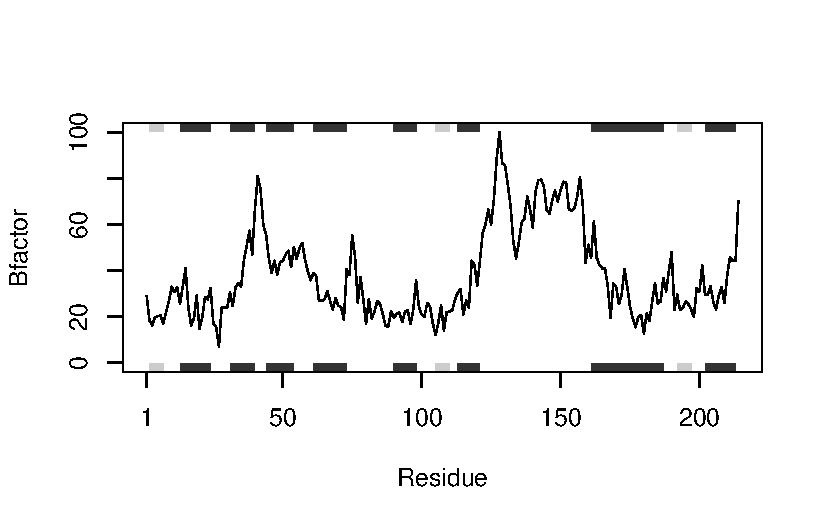
\includegraphics{hw6_turnin_files/figure-pdf/unnamed-chunk-7-1.pdf}

}

\end{figure}

\begin{figure}[H]

{\centering 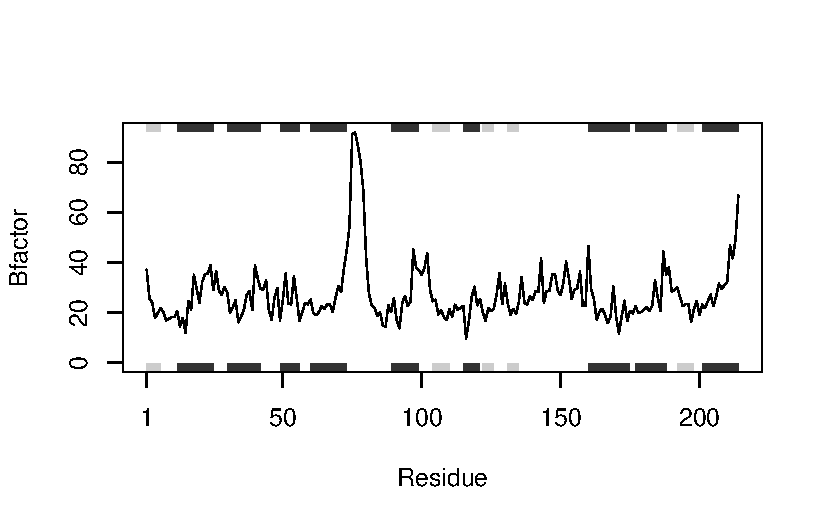
\includegraphics{hw6_turnin_files/figure-pdf/unnamed-chunk-7-2.pdf}

}

\end{figure}

\begin{figure}[H]

{\centering 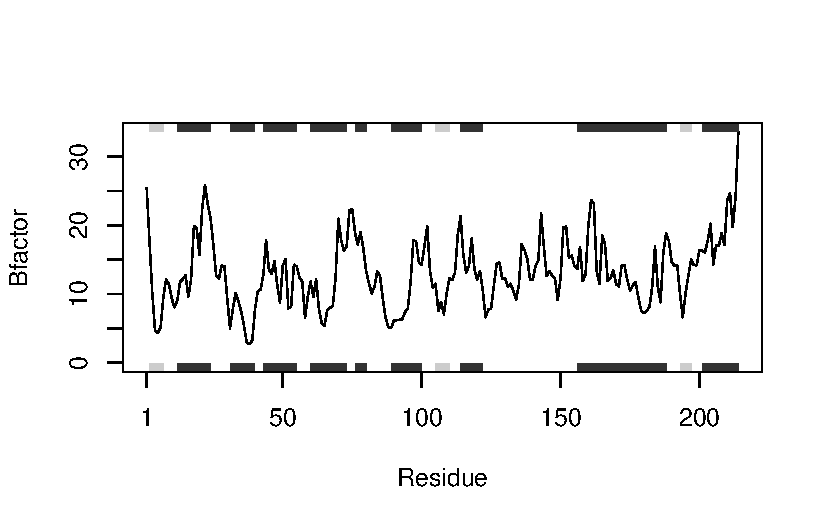
\includegraphics{hw6_turnin_files/figure-pdf/unnamed-chunk-7-3.pdf}

}

\end{figure}

\begin{Shaded}
\begin{Highlighting}[]
\CommentTok{\# As you can see, our function properly executes and our data and plots are displayed below for each protein. (our output)}
\end{Highlighting}
\end{Shaded}




\end{document}
